\documentclass[tikz,border=5pt]{standalone}
\usepackage{tikz}
\usetikzlibrary{positioning,arrows.meta}

\begin{document}
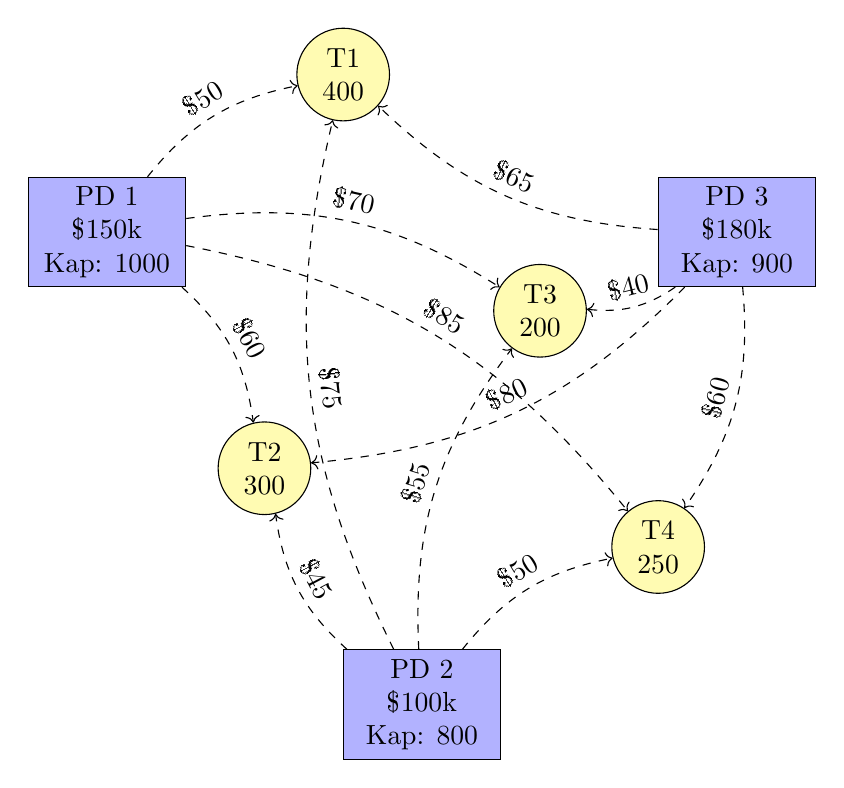
\begin{tikzpicture}[auto, node distance=8cm]

  % Simpul pusat distribusi (latar biru transparan, teks legap)
  \node[draw, rectangle, align=center, minimum width=2cm, minimum height=1cm, fill=blue, fill opacity=0.3, text opacity=1] (DC1) at (0,0) {PD 1\\ \$150k\\ Kap: 1000};
  \node[draw, rectangle, align=center, minimum width=2cm, minimum height=1cm, fill=blue, fill opacity=0.3, text opacity=1] (DC2) at (4,-6) {PD 2\\ \$100k\\ Kap: 800};
  \node[draw, rectangle, align=center, minimum width=2cm, minimum height=1cm, fill=blue, fill opacity=0.3, text opacity=1] (DC3) at (8,0) {PD 3\\ \$180k\\ Kap: 900};

  % Simpul toko (latar kuning transparan, teks legap)
  \node[draw, circle, align=center, minimum size=1cm, fill=yellow, fill opacity=0.3, text opacity=1] (S1) at (3,2) {T1\\400};
  \node[draw, circle, align=center, minimum size=1cm, fill=yellow, fill opacity=0.3, text opacity=1] (S2) at (2,-3) {T2\\300};
  \node[draw, circle, align=center, minimum size=1cm, fill=yellow, fill opacity=0.3, text opacity=1] (S3) at (5.5,-1) {T3\\200};
  \node[draw, circle, align=center, minimum size=1cm, fill=yellow, fill opacity=0.3, text opacity=1] (S4) at (7,-4) {T4\\250};

  % Koneksi PD1 ke toko dengan label biaya
  \draw[->, dashed] (DC1) to[bend left=20] node[midway, sloped, above] {\$50} (S1);
  \draw[->, dashed] (DC1) to[bend left=20] node[midway, sloped, above] {\$60} (S2);
  \draw[->, dashed] (DC1) to[bend left=20] node[midway, sloped, above] {\$70} (S3);
  \draw[->, dashed] (DC1) to[bend left=20] node[midway, sloped, above] {\$85} (S4);

  % Koneksi PD2 ke toko dengan label biaya
  \draw[->, dashed] (DC2) to[bend left=20] node[midway, sloped, above] {\$75} (S1);
  \draw[->, dashed] (DC2) to[bend left=20] node[midway, sloped, above] {\$45} (S2);
  \draw[->, dashed] (DC2) to[bend left=20] node[midway, sloped, above] {\$55} (S3);
  \draw[->, dashed] (DC2) to[bend left=20] node[midway, sloped, above] {\$50} (S4);

  % Koneksi PD3 ke toko dengan label biaya
  \draw[->, dashed] (DC3) to[bend left=20] node[midway, sloped, above] {\$65} (S1);
  \draw[->, dashed] (DC3) to[bend left=20] node[midway, sloped, above] {\$80} (S2);
  \draw[->, dashed] (DC3) to[bend left=20] node[midway, sloped, above] {\$40} (S3);
  \draw[->, dashed] (DC3) to[bend left=20] node[midway, sloped, above] {\$60} (S4);

\end{tikzpicture}
\end{document}
